\chapter{Pruebas}

En el capítulo anterior, se proporcionaba una visión sobre la implementación realizada, en este capítulo procederemos a mostrar que todo lo implementado se encuentra en funcionamiento.

\section {Pruebas unitarias}
Para la realización de las pruebas unitarias hemos hecho uso de Jest, una suite de test que integra numerosas herramientas. Para llevar a cabo la ejecución de los test usaremos la orden npm test, que ejecutará todos los archivos *.test.js. Dentro de estos archivos encontramos una líneas que indican los nombres de los tests (describe) y una serie de líneas que empiezan con la función test, dentro de las cuales se ejecutan y se evalúan las pruebas definidas.

Una vez ejecutamos los test obtendremos una serie de salidas, en las cuales se indica el éxito \ref{fig:testok} o el fallo de los test, y además en caso de fallo, se incluye una descripción de cuál ha sido la causa de este \ref{fig:testfail}.
\begin{figure}
  \begin{center}
    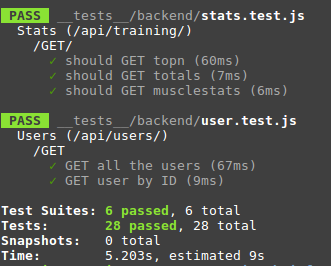
\includegraphics[width=\textwidth]{imagenes/test_pass.png}
    \caption{Test correctos}
    \label{fig:testok}
  \end{center}
\end{figure}
\begin{figure}
  \begin{center}
    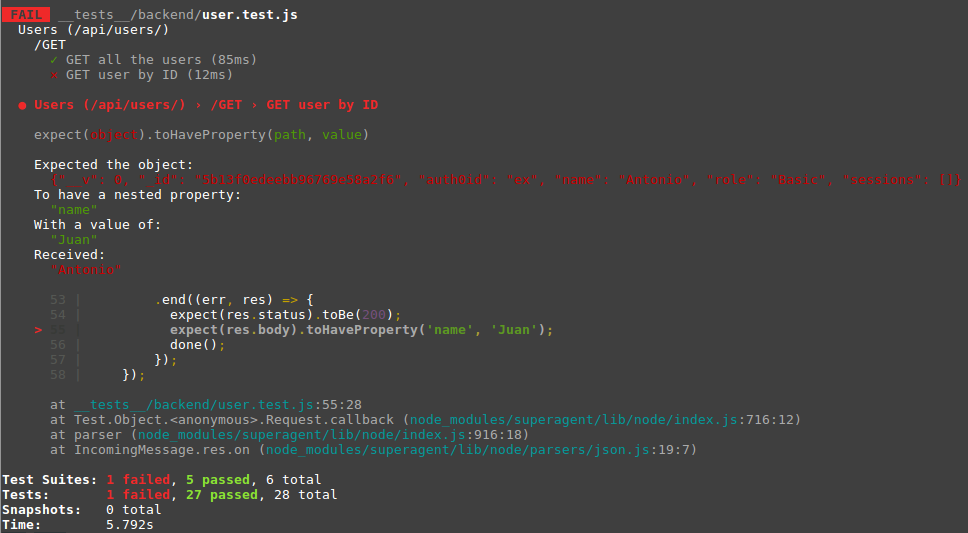
\includegraphics[width=\textwidth]{imagenes/test_fail.png}
    \caption{Test con fallos}
    \label{fig:testfail}
  \end{center}
\end{figure}
\section {Pruebas de cobertura}
Para las pruebas de cobertura también se ha hecho uso de Jest. Para la ejecución de estas pruebas hacemos uso de la orden npm run test-cov, esta ejecución consiste en realizar los test anteriores y comprobar que líneas ha sido cubiertas por ellos. Una vez finalizada la ejecución, se proporciona un resumen por pantalla \ref{fig:cob} y además se genera un informe mucho más detallado en formato HTML , en el cual podremos ver con todo lujo de detalles \ref{fig:cobd} cuáles líneas han sido testeadas y cuáles de ellas no.

\begin{figure}
  \begin{center}
    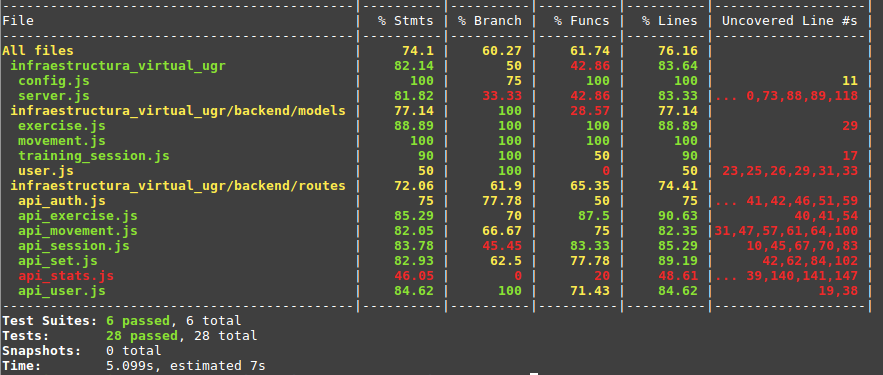
\includegraphics[width=\textwidth]{imagenes/cov.png}
    \caption{Visión test de cobertura}
    \label{fig:cob}
  \end{center}
\end{figure}
\begin{figure}
  \begin{center}
    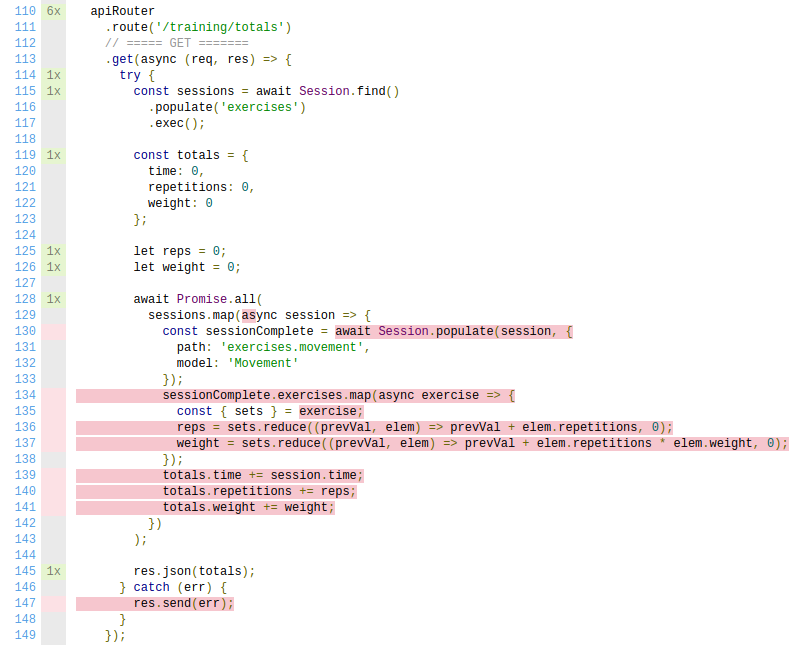
\includegraphics[width=\textwidth]{imagenes/cov_detail.png}
    \caption{Detalles test de cobertura}
    \label{fig:cobd}
  \end{center}
\end{figure}

\section {Integración continua}
Una vez que disponemos de los test unitarios y nuestro archivo NPM tiene las órdenes indicadas para ejecutarlos, la integración con Travis CI es muy sencilla. Para comprobar que todo funciona como debe, nos dirigimos a la web de Travis, y hacemos un push al repositorio, tras lo que podremos observar que los test empiezan a ejecutarse \ref{fig:travis}, confirmando con ello la correcta configuración. \ref{fig:travis2}

\begin{figure}
  \begin{center}
    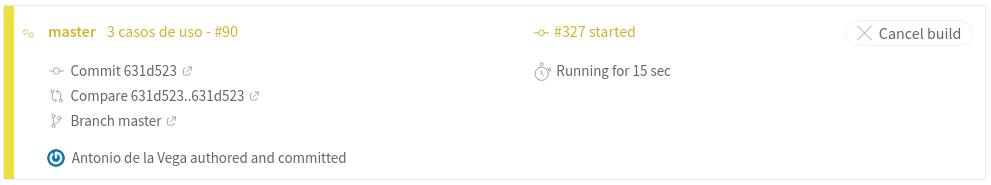
\includegraphics[width=\textwidth]{imagenes/init_travis.png}
    \caption{Inicio Travis}
    \label{fig:travis}
  \end{center}
\end{figure}
\begin{figure}
  \begin{center}
    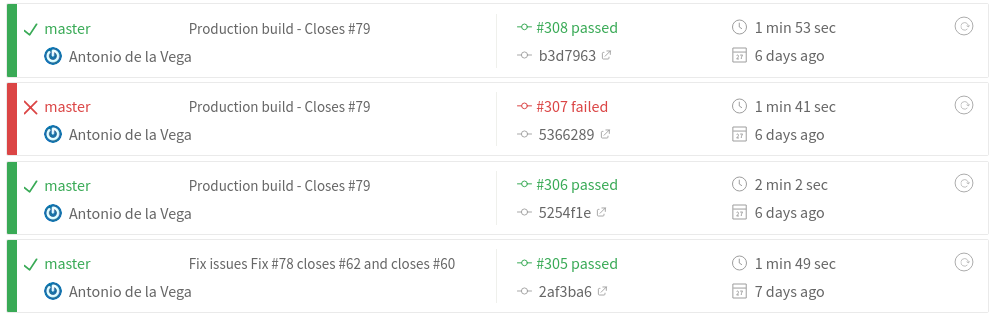
\includegraphics[width=\textwidth]{imagenes/travis.png}
    \caption{Resultados Travis}
    \label{fig:travis2}
  \end{center}
\end{figure}


\section {Despliegue automático}
Para el despliegue automático hemos hecho uso de Heroku, y con el objetivo de comprobar que todo está configurado de la forma correcta, nos dirigimos a la correspondiente web. Una vez ahí, hacemos un push a nuestro repositorio, y tras esperar a que Travis CI verifique los test, comenzamos a ver cómo se produce un nuevo \gls{build} y seguidamente un nuevo despliegue \ref{fig:heroku}, confirmando así que todo funciona de manera adecuada.


\begin{figure}
  \begin{center}
    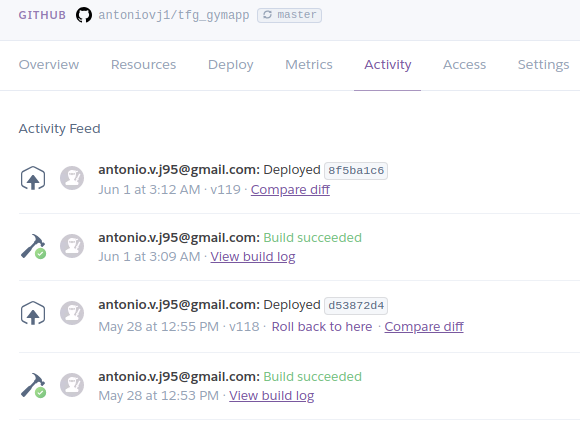
\includegraphics[width=\textwidth]{imagenes/heroku.png}
    \caption{Actividad Heroku}
    \label{fig:heroku}
  \end{center}
\end{figure}

\section {Contenedores}
También hemos comprobado que los contenedores se ejecutan correctamente, y a continuación en la figura, se muestra como comienza la ejecución sin errores. \ref{fig:docker}
\begin{figure}
  \begin{center}
    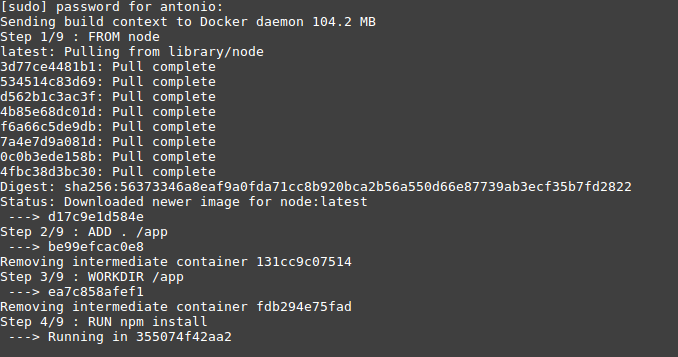
\includegraphics[width=\textwidth]{imagenes/docker.png}
    \caption{Primeros pasos Docker}
    \label{fig:docker}
  \end{center}
\end{figure}

\section {Provisionamiento}
\section {Despliegue Cloud}
\section {Acceso web y autenticación}
